\documentclass{article}
\usepackage[margin=1.1in]{geometry}
\usepackage{undertilde, amsmath, amsfonts, commath, cancel, graphicx}
\usepackage{accents}

\newcommand{\ut}[1]{\underaccent{\tilde}{#1}}

\title{PHYS 7125 Homework 5}
\author{Wenqi He}
\begin{document}
\maketitle
\section{}
The total proper time along a curve $\gamma$ is
\begin{align*}
\tau_{total} &= \int_\gamma d\tau = \int_\gamma \sqrt{-ds^2} 
= \int_\gamma \sqrt{-\Big(\frac{2M}{r} - 1\Big)dt^2 + \Big(\frac{2M}{r} -1 \Big)^{-1} dr^2 - r^2d\Omega^2}
\end{align*}
Inside the event horizon, $r < 2M$, the first and third term in the square root are negative, therefore
\begin{align*}
\tau_{total} &< \int^{2M}_0 \sqrt{\Big(\frac{2M}{r} -1 \Big)^{-1}} dr  \\
&= \Bigg[ -\sqrt{r(2M-r)} + 2M\cot^{-1}\left(\sqrt{\frac{2M}{r}-1} \right) \Bigg] \Bigg\rvert^{2M}_0 = \pi M
\end{align*}
\section{}
\subsection*{a}
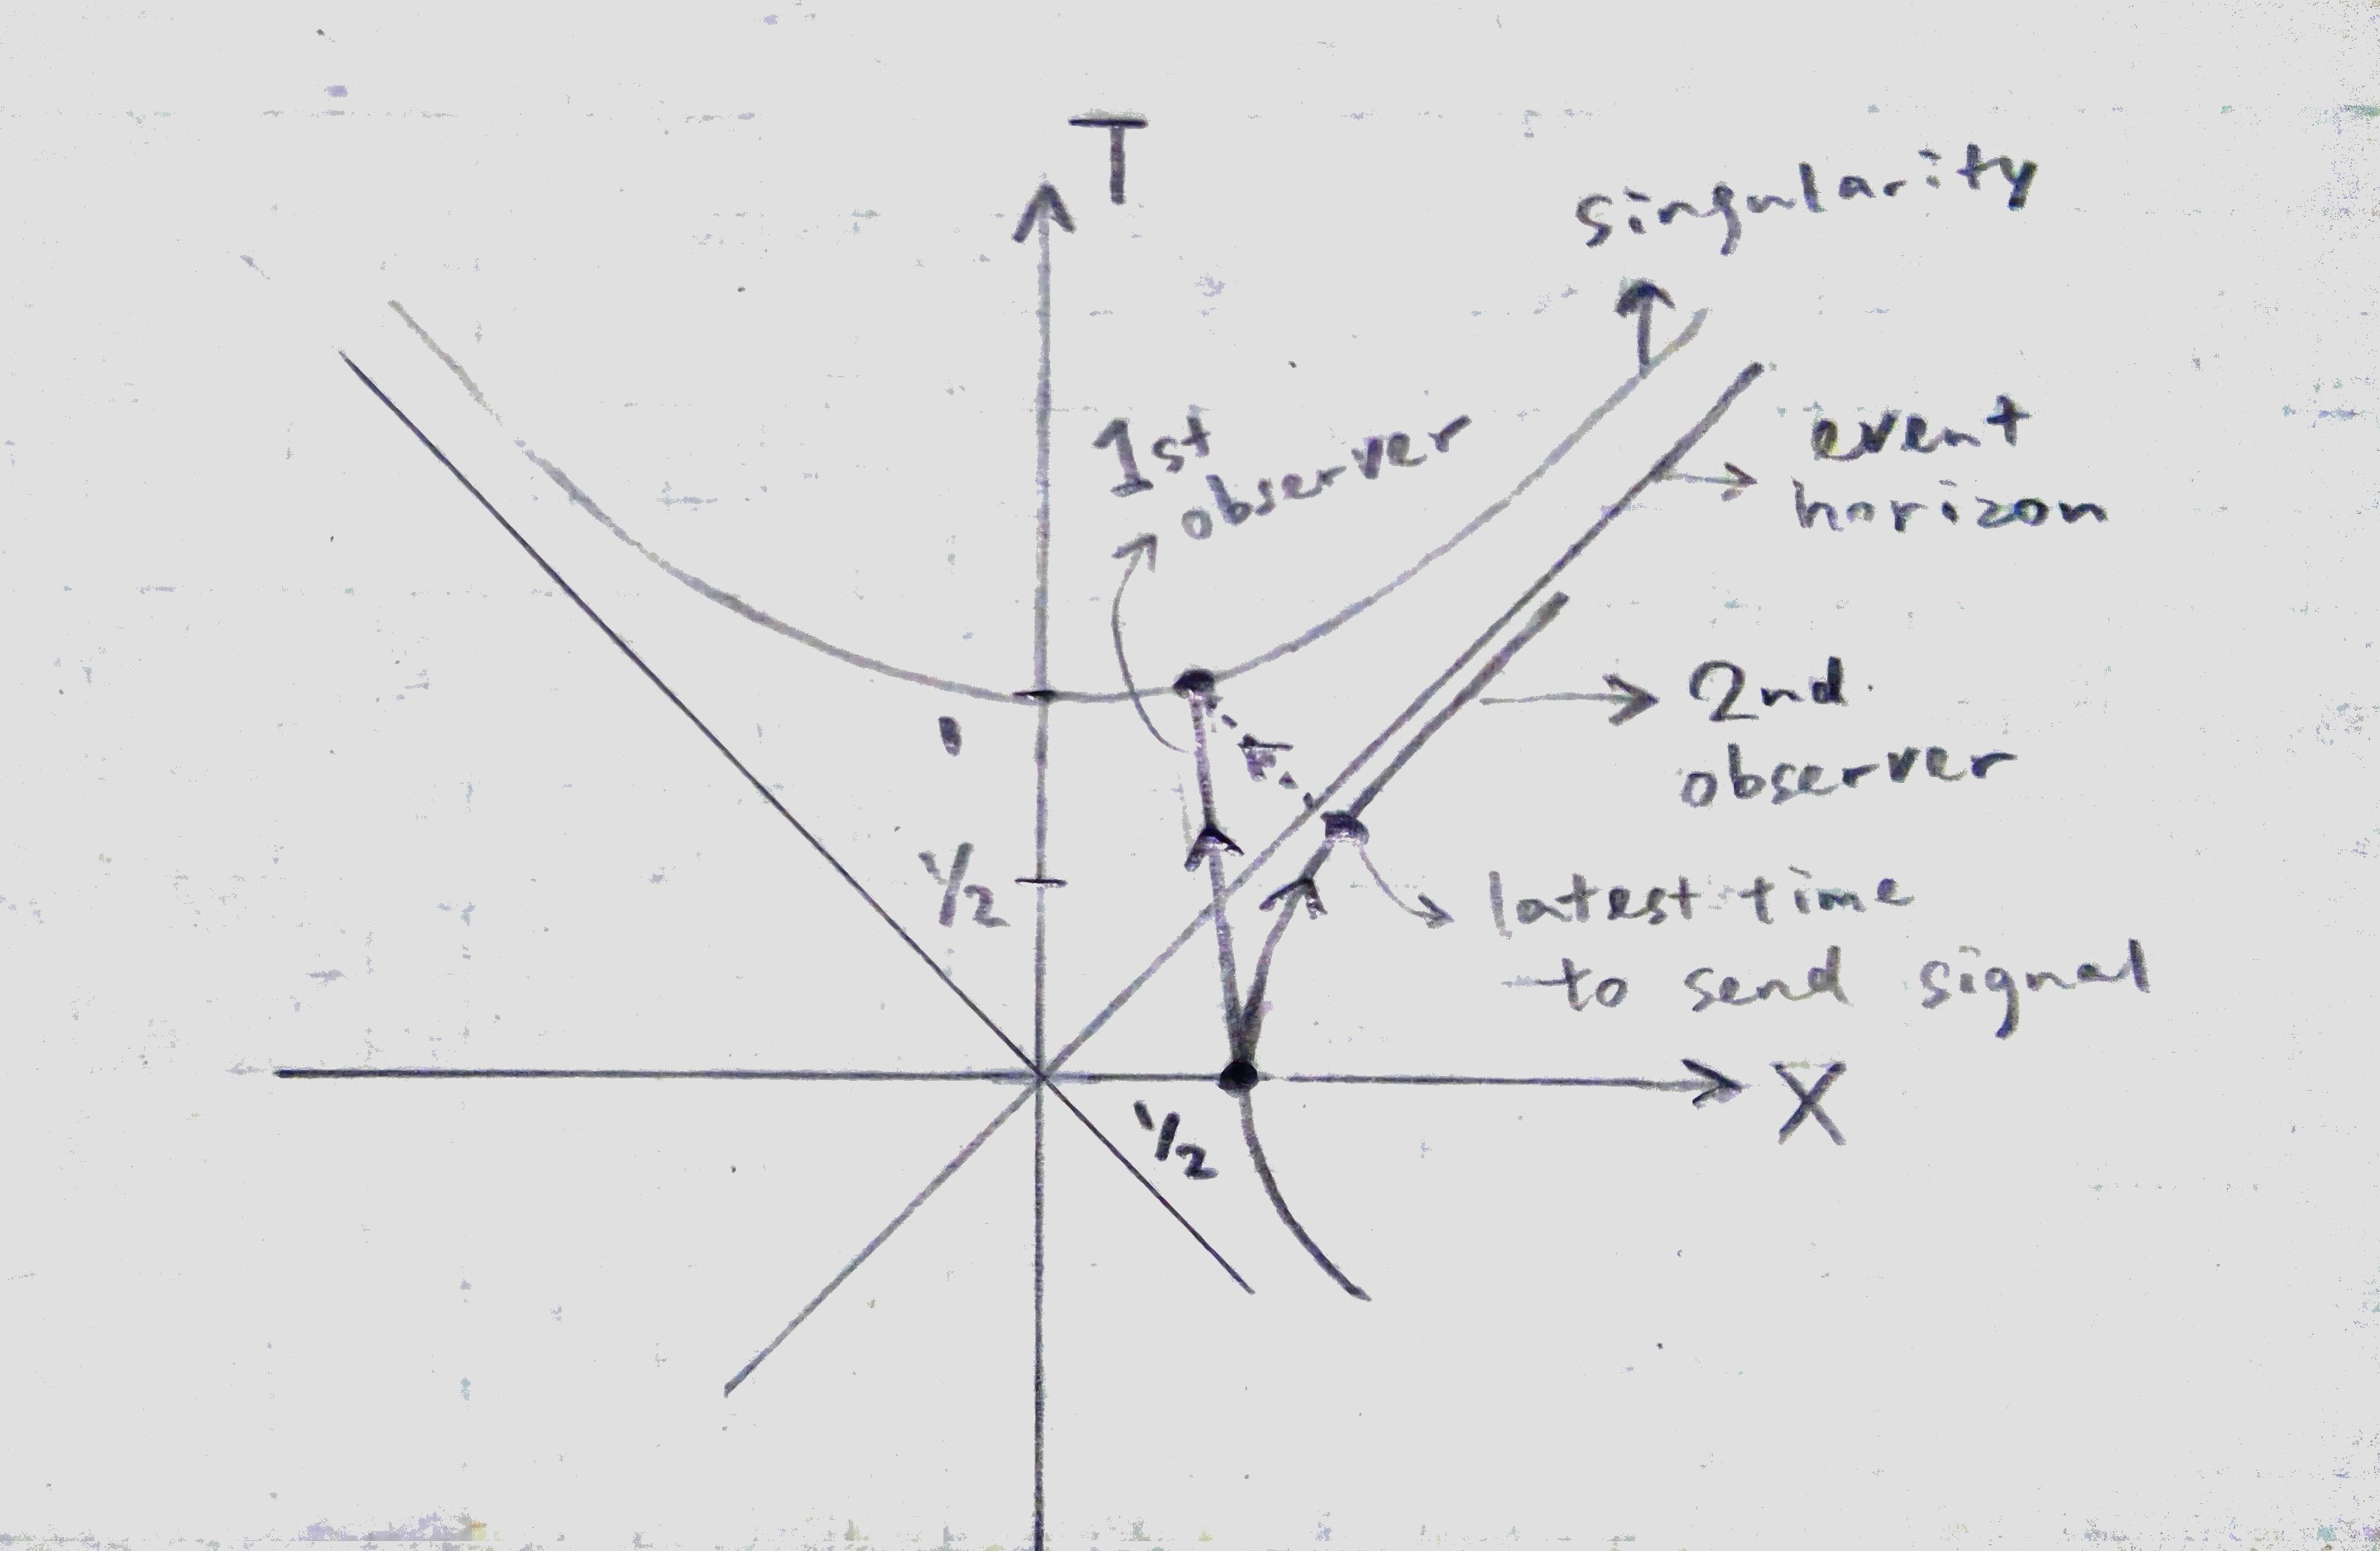
\includegraphics[width=\textwidth]{diagram.jpg}
\subsection*{b}
Yes, because the observer is massive. (If not, the light signal in (c) could never reach the falling observer, because the two worldlines would be parallel straight lines in a Kruskal diagram.)
\subsection*{c}
At constant $r = R$,
\[  T = \frac{1}{2}\sinh\left( \frac{t}{4GM} \right), \quad X = \frac{1}{2}\cosh\left( \frac{t}{4GM} \right)
	,\quad 4X^2 - 4T^2 = 1 \]
At $t = 0$ on this worldline,
\[ T = \frac{1}{2}\sinh0 = 0, \quad X = \frac{1}{2}\cosh0 = \frac{1}{2} \]
At the singularity,
\[ T = \cosh\left( \frac{t}{4GM} \right),\quad X = \sinh\left( \frac{t}{4GM} \right), \quad T^2 - X^2 = 1 \]
A timelike straight line passing through $(1/2, 0)$ can be expressed as 
\[ X = kT + \frac{1}{2}\]
where $-1 < k< 1$. When the first observer reaches singularity,
\[ (1- k^2)T^2 - kT - \frac{5}{4} = 0 \quad\Rightarrow\quad \boxed{T_s = \frac{k + \sqrt{5-4k^2}}{2(1-k^2)},\quad
	X_s = \frac{k^2 + k\sqrt{5-4k^2}}{2(1-k^2)} + \frac{1}{2}}\]
To reach this critical point, the photon emitted by the second observer must follow the straight line
\[ X  = - T + T_s + X_s \]
The photon's worldline in the past intersects the second observer's worldline at
\[ \cancel{4T^2} + 4(T_s + X_s)^2 -8(T_s+X_s)T - \cancel{4T^2} = 1\]
\[ \Rightarrow T = \frac{1}{2}\sinh\left( \frac{t}{4GM} \right)  = \frac{4(T_s+X_s)^2 - 1}{8(T_s + X_s)}
	,\quad \boxed{t = 4GM\sinh^{-1}\left(\frac{4(T_s+X_s)^2 - 1}{4(T_s + X_s)}\right)} \]
which is the latest Schwarzschild time at which the second observer could send the signal. If the worldline of the first observer is vertical in the Kruskal diagram, i.e. $k=0$, then $t \approx 4.70GM$
\section{}
A perfect fluid is incompressible, therefore $\nabla_\mu \rho = \partial_\mu \rho = 0$. From the continuity equation,
\[ \nabla_\mu(\rho u^\mu) =  \rho \nabla_\mu u^\mu = 0 \quad\Rightarrow\quad \nabla_\mu u^\mu = 0\]
Since the covariant divergence of the stress-energy tensor must vanish,
\begin{align*}
\nabla_\mu T^\mu{}_\nu &= (\nabla_\mu p + \cancel{\nabla_\mu\rho}) u^\mu u_\nu + (p+\rho) \cancel{(\nabla_\mu u^\mu)} u_\nu + (p+\rho) u^\mu (\nabla_\mu u_\nu) + \delta^\mu_\nu \nabla_\mu p \\
&=  u_\nu (\nabla_{\ut{u}} p)  + (p+\rho) \nabla_{\ut{u}} u_\nu + \nabla_\nu p \\
&= 0
\end{align*}
The free index $\nu$ can be dropped, yielding
\[ (p + \rho)\nabla_{\ut{u}}\ut{u} = - \nabla p - \ut{u}\nabla_{\ut{u}}p \]

\end{document}